\documentclass[a4paper]{report}
\usepackage{amsmath} 
\usepackage{graphicx}
\usepackage[utf8]{inputenc}
%\usepackage{geometry}
%\geometry{a4paper, top=3cm, bottom=3cm, left=3.5cm, right=3.5cm}
\DeclareUnicodeCharacter{2212}{-}
\title{DDPG + HER in FetchPush-v1 Gym Environment with Python3 and Tensorflow 2.0}
\author{Simone De Angelis 1760464\\ Veronica Romano 1580844}
\date{\today}


\begin{document}

\maketitle
\begin{abstract}
The purpose of this report will be to reproduce the results obtained in \cite{her} on a specific environment among the many presented in \cite{her}. First of all, we expose how the environment is represented and how our algorithm interacts with it. After that we highlight the differences between Deep Q-learning and Deep Deterministic Policy Gradient, focusing  on the general principles of DDPG combined with Hindsight Experience Replay.
The second part of the paper shows the results obtained following the same training procedure exposed in \cite{her} and a diffent one that will be explained in the corresponding section.
\end{abstract}
\chapter{Introduction and Work Purposes}
Reinforcement Learning is learning what to do and how to map situations to actions. The end result is to maximize the numerical reward. The learner is not told which action to take, but instead must discover which action will yield the maximum reward. As illustrated in Figure \ref{Fig: scheme}, an agent starts from a state $s_t$ and by choosing actions $a_t$ according to  a certain policy $\pi$ interacts with the environment that gives back to it  a reward $r_{t+1}$ and a new state $s_{t+1}$.

\begin{figure}[h!]
\centering
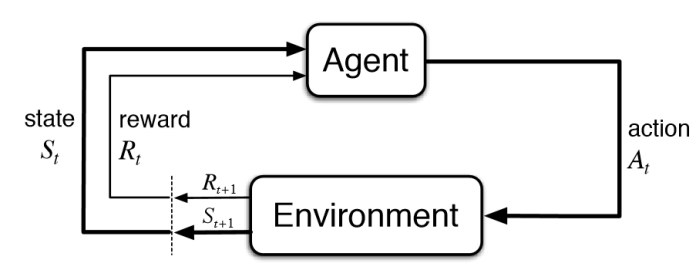
\includegraphics[scale=0.5]{reinforcement.jpg}
\caption{\label{Fig: scheme} Formulation of a basic Reinforcement Learning project.}
\end{figure}

This cycle proceeds until either a terminal condition or a goal is reached. 

\section{Environment and Tools}
We used OpenAI Gym environment combined with MuJoCo. In the past there weren't many standard environments that could be used to develop reinforcement learning algoirthms. In fact with the rise of OpenAi, reinforcement learning has become more practical and implementable with respect to previous  reinforcement learning methods. Gym is available on the corresponding GitHub repository and allows to use any of the environment present in the repository for free, from atari games to Robotic arms environemnt. The Fetch environment needs MuJoCo (Multi-Joint dynamics with Contact) that is an engine simulating real and detailed rigid body simulation with contacts forces. Mujoco-py is the library needed in order to work with tha gym environment, since it only supports python3 as programming language. However the best part is that MuJoCo provides the physical interactivity (like calculation of contact forces) which helps an engineer or researcher to test their model rigorously before moving to production.
\begin{figure}[h!]
\centering
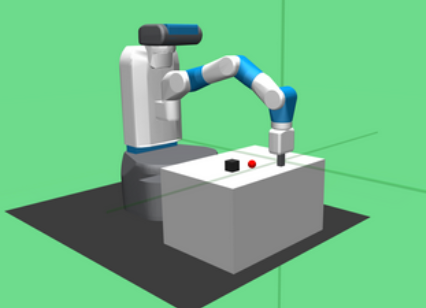
\includegraphics[scale=0.9]{fetchpush.png}
\caption{\label{Fig: fetchpush} FetchPush-v1 Gym environment.}
\end{figure}

The Fetch environment is based on the 7-DoF Fetch robotics arm which has a two-fingered parallel gripper that are locked to prevent grasping in the push task. The learned behavior is usually a mixture of pushing and rolling. The observation space is a dictionary object containing  
\begin{itemize}
\item observation: It's an array of 25 elements containing the cartesian position of the end effector, cartesian position and orientation of the desired object, its linear velocity as well as the position and linear velocity of the robot's gripper.
\item desired\_goal: The goal that the agent has to achieve. In FetchPush-v1 is the 3-dimensional target position on which we would like the box to be and it's represented by the red point in \ref{Fig: fetchpush}
\item achieved\_goal: The goal that the agent has currently achieved represented by the black box in figure \ref{Fig: fetchpush}.
\end{itemize}


Rewards by default are sparse and binary: the agent obtains a reward of 0 if the object is at the target location and −1 otherwise. 
\chapter{Implementation Assignment \label{ddpgalgo}}

\section{DDPG + HER Algorithm}
Deep Deterministic Policy Gradient (DDPG) (illustrated in \cite{ddpg}) is a model-free, off-policy actor-critic algorithm using deep function approximators to learn policy in continuos action spaces. In the next subsections we will give the intuition about vanilla DDPG without focusing too much on all the details. After that, we will expose how Hindisght Experience Replay interact with a DDPG algorithm. 
\subsection{DDPG (Deep Deterministic Policy Gradient)}
DDPG is deterministic in the sense that the policy $\mu $ maps states to action directly
\begin{equation}
\mu_d : S \rightarrow A \qquad \emph{such that} \qquad \mu_d(s) = a
\end{equation}
where $ S $ and $ A $ are the state and action space with $ s \in S$ , $a \in A$. Differently from a stochastic policy,  a deterministic policy, given a certain state, will always output the same action.
In order to understand  the algorithm, let's start by giving the definition of the action value function, also known as Q-value function:
\begin{equation}
Q^{\pi}(s) = E_{\mu} \{R_t \mid s_t, a_t  \} =  E_{\mu} \{\sum_{k}^{\inf} \gamma^k r_{t+k+1} \mid s_t, a_t  \}
\end{equation}
where $R_t$ is the infinite-horizon discounted reward. The Q-value function actually represent the expected return when following a certain policy $\mu$ (used to choose actions) starting from a certain state $s_t$ and action $a_t$ that was not taken according to policy $\mu$.
As in Deep Q-Learning, the Bellman equation represents the core of the whole algorithm:
\begin{equation} \label{bellman eq}
Q^*(s,a)=E_{s'\sim P} [r(s,a) + \gamma \max_{a'}(Q^*(s',a')]
\end{equation} 
The equation written in \ref{bellman eq} is the Bellman equation for the optimal action-value function and it is also used in Deep Q-learning. The main difference between the two methods is in how the max function in \ref{bellman eq} is computed: In Q-learning, since the action space is discrete, there is no problem in finding $a$ such that it maximizes the action value function. Even if it exist methods to actually discretize continuos action spaces, this approach often doesn't work due to what is known as the "curse of dimensionality". In few words, the discretization operation causes the action space to blow up, making the max operation computationally heavy and infeasible if we need it everytime the agent takes actions. DDPG exploits the fact that the action space is continuos and uses gradient based methods to compute the max operation we've seen above, since $Q(s,a)$ is differentiable with respect to $a$. Both in Deep Q-learning and in Deep Deterministic Policy Gradient, the "deep" word refers to the fact that the Q-value function is replaced by an apporixamator $Q_{\phi}^{*}(s,a)$ represented by a deep neural network of parameters $\phi$ that are learned through the minimization of the Mean Bellman squared error, MBSE:
\begin{equation} \label{mbse eq}
L(\phi, \textit{D}) = E_{s,a,r,s',d \sim \textit{D}}\biggl[\bigl(Q_{\phi}^{*}(s,a) - r(s,a) + \gamma(1-d)  \max_{a'}(Q^*(s',a')
\bigr)^2
\biggr]
\end{equation}
where $s,a,r,s',d \sim \textit{D}$ stands for a set \textit{D} of transitions. This set of transitions is stored in a replay buffer, that must be large enough to allow trainings between transiitions that must not be temporarly related in order to avoid overfitting to the most recent behaviors. This explains why we defined DDPG an off policy method. In order to compute the max operation, both Q-Learing and DDPG make use of target networks: Intead of computing $Q^*(s',a')$ with the current parameters $\phi$, the Q function is computed with a set of parameters that are close to the main network and are time-delayed. One of the difference with deep Q-learning is that the parameters of target networks $\phi_{targ} $ are soft-updated every time the main network gets updated following the rule:
\begin{equation} \label{soft update rule}
\phi_{targ} \leftarrow \tau \phi_{targ} + (1- \tau) \phi
\end{equation}
with $\tau$ being close to 1.\\
We previously mentioned how the main difference about the two networks stands in the way of computing tha max operation in \ref{mbse eq}. Since it is often unacceptable to compute it when the action space is large or continuos, DDPG firstly learns to find an approximator of policy $\mu_{\theta}$ by solving through gradient ascent
\begin{equation}
\max_{\theta}E_{s \sim D}[Q_{\phi}^*(s,\mu_{\theta}(s)]
\end{equation}
notice that the gradient will be computed just with respect to $\theta$. When solving this optimization problem, we're finding the policy $\mu_{\theta}$ that will return an action $a$ that mazimizes the Q-value function. Now it's clear how DDPG avoids computing the max operation in \ref{mbse eq}: in order to compute the parameters $\phi$ the loss function (MSBE) gets minimized via stochastic gradient descent
\begin{equation}
L(\phi, \textit{D}) = E_{s,a,r,s',d \sim \textit{D}}\biggl[\bigl(Q_{\phi}^{*}(s,a) - r(s,a) + \gamma(1-d) Q_{\phi_{targ}}(s, \mu_{\theta}(s))
\bigr)^2
\biggr]
\end{equation}
notice that $Q_{\phi_{targ}}$ that has replaced $ \max_{a'}(Q^*(s',a')$ is approximated with a target neural network which parameters are soft updated 
with the same rule of \ref{soft update rule}. It's worth mentioning that actions computed with $\mu_{\theta}(s))$ are different from the ones we're sampling from the replay buffer since the method is off-policy. Let's recap what we've seen so far. DDPG, being an actor-critic technique, consists of two models: Actor and Critic. The Actor is a policy neural network ($\mu_{\theta} $) that takes the state as input and outputs the exact action, the Critic $Q(s,a)$ is a Q-value neural network that takes state and action as input and outputs the Q-value. In order to get convergency of the algorithm, we've seen how target networks are implemented, causing the whole method to use 4 neural networks, even if the parameters of targets are not learned but just soft-updated.






\subsection{HER (Hindsight Experience Replay)}
Hindsight Experience Replay is a reinforcement learning algorithm that can be combined with any off-policy RL algorithm. In the next section we will show how DDPG combined with experience replay achieves high levels of success rate in the Fetch-Push task. The intuition that lies behind Hindsight experience replay is that even if we do not reach a specific goal when performing an action we can actually learn something from failure. This concept is as obvious as hard to understand for an agent receving only sparse and binary rewards. 
 A classical reinforcement algorithm will not learn anything from this experience since it just obtains a constant reward equal to -1, that does not contain any learning signal. HER allows to learn also from this type of experiences. Even if we have not succeeded at a specific goal, we have at least achieved a different one. We can imagine that we want to reach this new goal at the beginning instead of that we want to achieve originally. By doing this substitution, the reinforcement learning algorithm can obtain a learning signal since it has achieved some goal; even if it wasn't the one that we meant to achieve originally. If we repeat this process, we will eventually learn how to achieve arbitrary goals, including the goals that we really want to achieve. This technique is called Hindsight Experience Replay because it replays experience with goals which are chosen in hindsight, after the episode has finished. The complete algorithm of HER is illustrated in Figure \ref{Fig: her}. The authors of \cite{her} have also shown how HER works better when dealing with sparse and binary rewards rather than with shaped ones: they actually motivate these results by asserting that optimizing shaped rewards may not coincide whith the success condition. Further from that, shaped rewards such as the distance between the goal and the box in the Fetch-push environment may penalize too much behaviors that we actually want to achieve (touching the box but moving it away from the goal).

\begin{figure}[h!]
\centering
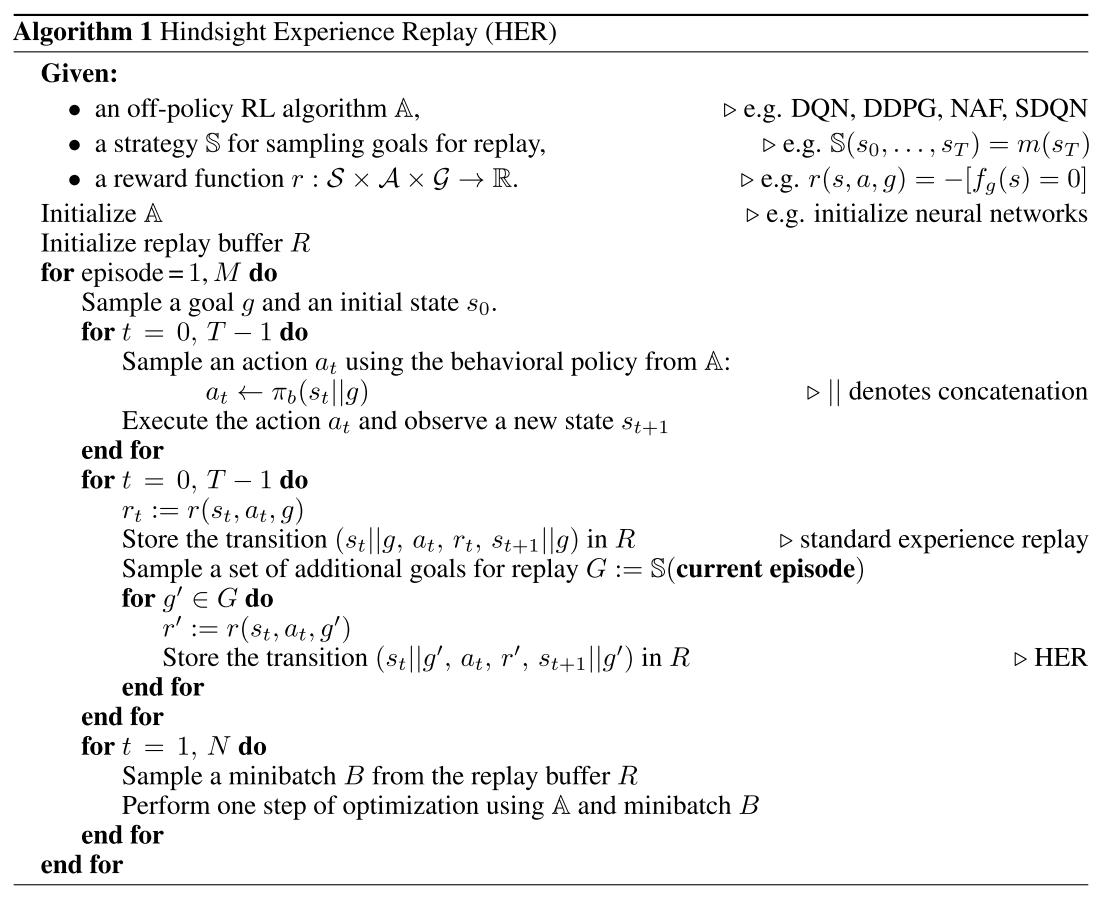
\includegraphics[scale=0.5]{her.png}
\caption{\label{Fig: her} Pseudocode of HER algorithm.}
\end{figure}
As shown in figure \ref{Fig: her}, the algorithm is as simple as effective: whenever we take an action during the training, we store the corresponding transition $(s_t \mid\mid g , a_t, r_t, s_{t+1}\mathbin\Vert g)$ in the replay buffer. Note that $s_t \mid \mid g$ denotes concatenation: when implementing Hindsight experience replay we're always giving concatenation of state and goal as input to both the actor (Policy) and critic (Q-value) networks. 
 After that, we sample from the transitions of the episode we've run a certain number (k) of additional goals and we compute the reward function applied to each of this new goal and store in the replay buffer the corresponding transition . The number k can be seen as the ratio of data coming from HER to the replay buffer since it is the number of "HER" transitions stored in the replay buffer . The way we choose how to sample goals defines the strategy of the Hindisght experience replay method:
\begin{itemize}
\item \textit{future}  replays with k random states which come from the same episode as the transition being replayed and were observed after it
\item \textit{episode}  replays with k random states coming from the same episode as the transition being replayed
\item \textit{random}  replays with k random states encountered so far in the whole training procedure
\end{itemize}
In this work we tried do reproduce the results of the episodic strategy trying out different values of k. We also tried to implement a different strategy that is not mentioned in the original paper. In the paper is shown that all these strategies excluded the \textit{random} one are able to solve pushing task regardless the value of k.








\chapter{Experiments and Results \label{exp}}

As previously  mentioned, our work consisted of exploring in FetchPush-v1 environment, implementing the algorithm DDPG+HER. To implement our work we write a code in Python3 and TensorFlow 2.0. The code is structured in this way:

\begin{itemize}
\item a \textit{buffer.py} file in which is implemented the replay buffer with high dimension in which the transitions are stored through the use of agent function \textit{remember()}. These transitions include state, action, reward, new state reached after implementing an action, a flag \textit{done} which indicates if the goal is reached and the goal. These stored transitions will be then used to define the new goals for HER implementation. In this file is also defined a function called \textit{sample\_buffer()} which is used in DDPG implementation for sampling a random minibatch of N transitions from the replay buffer.

\item a \textit{ddpg\_tf2.py} file in which all the parameters for the agent are defined and the DDPG algorithm is implemented. Here are also initialized the target actor and target critic networks with the parameters reported in Table \ref{table}, size of the replay buffer, the value of the discount factor $\gamma$, the value for updating the target networks $\tau$ and also the noise is set. It is used for adding noise to the policy for the choice of the action to execute. In this file are also created the actor and critic target networks by coping the original actor and critic networks. To each of the for networks is applied an Adam optimizer with different learning rate for the actor and critic networks. Here are defined a function for updating the network parameters that takes tau as input and implement the last stage of the pseudocode of DDPG algorithm, a remember function for storing the transitions, a function for saving and one for loading the models of the networks. In the file is also defined a function for choosing an action which takes as input the state and the goal, concatenate these as illustrated in the pseudocode of HER and gives it to the actor which computes the policy for choosing the action. This function returns the action. The last function defined is the learning function, in which the critic network is updated by computing the target and applying the Mean Squared Error loss. While the actor network is updated by applying the gradient ascendant. this permits to update the networks parameters.


\item a \textit{networks.py} file in which the actor and critic networks are created by following the conventional parameters used in this kind of tasks found on several papers regarding this argument (also reported in Table \ref{table}). The networks are created by using \textit{tensorflow.keras} and are formed by only dense layers with \textit{relu} as activation function, and a final critic dense output layer without activation function, and a final actor dense output layer with \textit{tanh} as activation function. Moreover the weights of the networks for training are saved in 2 files with extension \textit{.h5}, one for the critic network and one for the actor network. the critic network will return the Q function, while the actor network will return the policy $\mu$.



\item a \textit{main\_ddpg.py} file in which the environment is imported. To the agent, so the DDPG algorithm, are provided the environment, the dimension of the \textit{observation} space as input dimension, the dimension of the \textit{desired\_goal} and the \textit{action\_space} dimension. this file is created by following the stages of the pseudocodes as deeply illustrated in Chapter \ref{ddpgalgo}.

\end{itemize}

All the parameters we have used are taken from literature works and from the papers cited in the Bibliography. In the following section the performed experiments are deeply explained. The following Table \ref{table} reports all the parameters used for all the experiments while the changed parameters will be illustrated in the specific section.
\\

\begin{table}[h]
\begin{center}
\begin{tabular}{|l|r|} 



\hline

\multicolumn{2}{|c|}{}\\
\multicolumn{2}{|c|}{\textbf{\Large            Parameters Table}}\\
\multicolumn{2}{|c|}{}\\

\hline

FC layers Critic 			& 2			\\
FC Critic dimensions		& 512		\\
Learning Rate Critic 		& 0.002		\\
FC layers Actor 			& 2			\\
FC Actor dimensions 		& 512		\\
Learning Rate Critic 		& 0.001		\\
Discount factor $\gamma$	& 0.99		\\
Update factor $\tau$		& 0.005		\\	%or 1?
Noise						& 0.1		\\
Replay Buffer dimension		& 1000000	\\

\hline
\end{tabular}
\end{center}
\caption{\label{table} Table of the parameters used for all the experiments}
\end{table}


\section{Experiments and Plots}
We performed some experiments changing the way in which HER is implemented.
First of all we implemented first only the DDPG algorithm but as we expected this provided no good results. Then we added also HER. In this experiment we implement a  sort of \textit{episode} HER. It takes k random states from the same episode and replays them as the transition being replayed. We perform this in two ways, by taking the first 24 states of the same episode and the last 24 states of the same episode. They are not randomly taken. We performed a learning with 60000 episodes, and each episode is formed by 50 iterations or steps. During these iterations we evoked the learning function from the agent class each time also if the robotic arm didn't still reached the goal, so when \textit{done=False} and after adding the current transition to the replay buffer. If the robot reached the goal and so \textit{done=True}, we increased the success rate. While for each episode, after iterating all the 50 steps, if the robot has not still reached the goal and so \textit{done=False}, we take the final box position from the state (these are the third, forth and fifth components of the state). At this point if the HER condition is verified, such that the distance between the final box position and the initial box position is less or equal than 0.05, for each of the 24 states taken from the beginning or from the end, we take a random stored position for the box in the current episode. Now if the final box position is more close to the goal than to the starting position, we stored this transition with the random position of the box, and we perform the learning. However the learning is performed also if the last condition is not verified and so for each of the 24 transition considered. This because we consider the fact not only that the box is near to the goal but also the fact that the end-effector of the robotic arm has moved the box. As we can see the learning produces good results reaching a success around 90\% both by considering the first and the last 24 stored transition. However we have to mentioned that the training by considering the first 24 transitions is faster that the one that considers the last 24 transitions. In the Table \ref{exp1} are reported the specific parameters used for the first two experiments. The results are illustrated in Figure ? and Figure ?.


\begin{table}[h]
\begin{center}
\begin{tabular}{|l|r|} 



\hline

\multicolumn{2}{|c|}{}\\
\multicolumn{2}{|c|}{\textbf{\large       Experiment 1 Parameters Table}}\\
\multicolumn{2}{|c|}{}\\

\hline

Batch Size 					& 64			\\
Number of episodes			& 60000			\\
k							& 24 (first and last)	\\


\hline
\end{tabular}
\end{center}
\caption{\label{exp1} Table of the specific parameters used for the first two experiments.}
\end{table}

For the second groups of experiment we try to change the parameter k that establish the number of states taken for replaying but we also changed the training procedure. By following more strictly the training procedure in \cite{her} (in detail what explained in Appendix A) we perform a training with 200 epoches and each epoch is formed by 50 cycle and each cycle by 16 episodes. In this way each epoches contains $16 * 50=800$ iterations. The concept is the same of the previous experiments but in this case the learning is performed only if the robotic arm effectively reach the goal. In fact the end of each cycle are performed 40 optimization steps in which the learning takes place. In this case a real episodic HER is implemented. We started by taking 8 random box stored positions and then if, for each of them, the condition that the random box position is closer to the goal with respect the initial position (it means that the box has been moved toward the goal), we stored this current transition. However as previously mentioned the learning is done only at the end of each cycle. Also this approach works, in fact as mentioned in \cite{her} for each value of k in the episodic HER we can obtain good results. The problem of this approach is that, because it takes random transitions from the replay buffer and so random position for the box, the results can vary significantly. In fact we reached very different results as we can see from the plots in figure ?; in different experiments with the same parameters, sometimes the robot doesn't learn and sometimes it reached a success equal to 92\% or equal to 78\% (reported in Figure). The Table \ref{exp2} is a report of the parameters used for this experiment.


\begin{table}[h]
\begin{center}
\begin{tabular}{|l|r|} 



\hline

\multicolumn{2}{|c|}{}\\
\multicolumn{2}{|c|}{\textbf{\large    Experiment 2 Parameters Table}}\\
\multicolumn{2}{|c|}{}\\

\hline

Batch Size 					& 128			\\
Number of Episodes			& 16			\\
Number of Cycles			& 50			\\
Number of Epoches			& 200			\\
k							& 8				\\


\hline
\end{tabular}
\end{center}
\caption{\label{exp2} Table of the specific parameters used for the second experiment with k equal to 8 random transitions.}
\end{table}



\begin{thebibliography}{}

\bibitem{multigoal}
Plappert, Matthias, et al. "Multi-goal reinforcement learning: Challenging robotics environments and request for research." arXiv preprint arXiv:1802.09464 (2018).

\bibitem{her}
Andrychowicz, Marcin, et al. "Hindsight experience replay." Advances in neural information processing systems. 2017.

\bibitem{ddpg}
Lillicrap, Timothy P., et al. "Continuous control with deep reinforcement learning." arXiv preprint arXiv:1509.02971 (2015).

\end{thebibliography}


\end{document}